\subsubsection{IoT Protocols and Protocol Conversation}
Kubernetes was designed for the Inernet and not for the heterogenity of the edge. This means the IoT gateway must either implement a DHCP server, the IoT device must have a static IP or the communication is facilitate outside Kubernetes realm and then converted by a service to IP. Please note that lower level protocols for establishing a connection between two devices, e.g. Ethernet, Wi-Fi (IEEE-802.11) or Bluetooth, are not discussed at this point. The most common IoT protocols are MQTT, CoAP, AMQP and DDS. In contrast to Internet protocol stack, these technologies do not need to support legacy systems and can thus concentrate on whats important in IoT, very low energy, distribution and memory consumption. I will mainly compare MQTT\cite{MQTT50:online} to CoAP\cite{CoAP—Con75:online} because of the their vast usage and academic literature. \Cref{fig:mqttVsCoap} shows side by side the architecture of MQTT and CoAP. Both are based on machine to machine (m2m) communication and are optimized for the IoT space, but the similarities stop there.
\begin{figure}[h!]
    \centering
    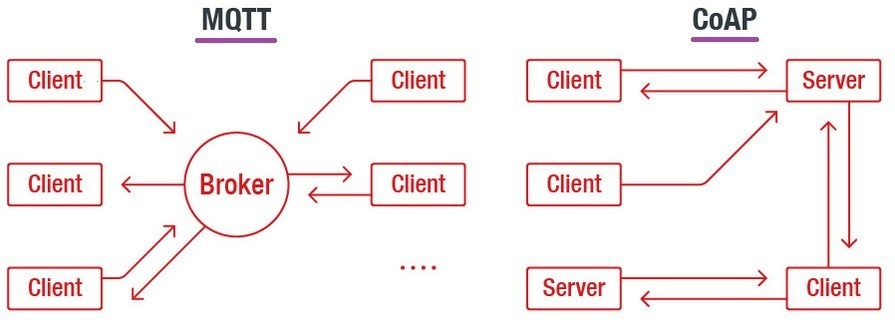
\includegraphics[scale=0.45]{figures/mqtt-vs-coap.jpg}
    \caption{MQTT and CoAP architecture side by side\cite{COAPvsMQTT27:online}.}
    \label{fig:mqttVsCoap}
\end{figure}
MQTT is based on the publish-subscribe massaging pattern which relies on a central entity, called broker, to enable communication between multiple nodes, mainly IoT devices. CoAP on the other side is a classic client server protocol and is based on the Internet stack. Researches compared the two standards and found "MQTT messages experienced lower delays than CoAP for lower packet loss and higher delays than CoAP for higher packet loss"\cite{MQTTvsCoAPAnalysisIEEE}. They also found that the message overhead for small messages is significantly lower at 25\% or less for CoAP compared to MQTT for reliable message transmission. Whereas in MQTT the broker needs additional services to convert the data to Internet compatible standards, CoAP is already able to communicate directly through the Internet. This opens up new possibilities including decentralized communication in subnets.\\
Finally, the data serialization can be even more important than the protocol itself. With the advent of RESTful services JSON soared in popularity. It is human readable but not very space efficient. When researches compared JSON to protobufs they found huge message size differences between the two, shown in \cref{fig:jsonVsProtobufs}.
\begin{figure}[h!]
    \centering
    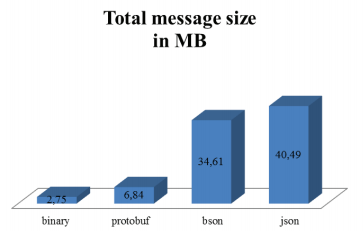
\includegraphics[scale=0.45]{figures/jsonVsProtobufs.png}
    \caption{Memory consumption of different serialization methods\cite{}.}
    \label{fig:jsonVsProtobufs}
\end{figure}
The researches conclude "the Protocol Buffers are a serious candidate for standardized way of communication in field of Internet of Things"\cite{jsonVsProtobufs}.